\section{Related Work}
\label{sec:related}

\paragraph{MPC languages and compilers.}
Languages and compilers for secure computation have seen significant advances in recent years. The early MPC compilers Fairplay~\cite{Ben-David:2008},
and Sharemind~\cite{Bogdanov:2008} were followed by PICCO~\cite{Zhang:2013}, Obliv-C~\cite{Zahur:2015}, TinyGarble~\cite{Songhori:2015},
Wystiria~\cite{Rastogi:2014}, and others. A new generation of MPC compilers
includes SPDZ/SCALE-MAMBA/MP-SPDZ~\cite{Keller:2020} and the ABY/HyCC/MOTION~\cite{Demmler:2015,Buscher:2018b,Braun:2022} frameworks.
These two families are the state-of-the art and
are actively developed. Another recent development is Viaduct~\cite{Acay:2021}, a functional language and compiler that supports a range of secure computation
frameworks, including MPC and ZKP. Hastings et el. present a review of compiler frameworks~\cite{Hastings:2019}. We believe that our work is unique as 
as it falls between the high-level language and lower-level circuit protocols.

\begin{comment}
While each of these languages and compilers brings in new ideas and advances, none addresses the problem of ``circuit independent'' intermediate
representation and optimization. We envision a classical compiler structure: (1) a Wysteria, Viaduct, Obliv-C, or IMP Source front end, including rich type systems and
AST-level semantic analysis, compile into the MPC Source IR, (2) MPC Source-level optimizations take place, followed by (3) back-end compilers into circuits.
Our focus is at the intermediate level.

%{\begin{center}
%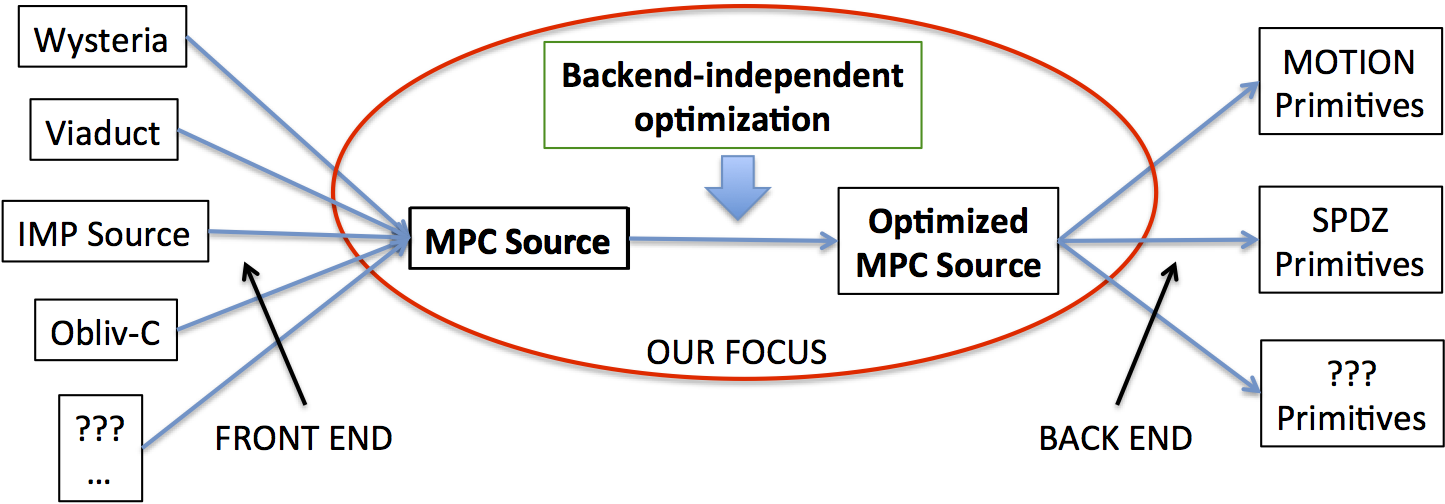
\includegraphics[width=0.5\linewidth]{figs/focus.png}
%\end{center}
%}

Many works focus on the implementation of MPC protocols exposing an API to the programmer. For example, the ABY/MOTION line of
compiler frameworks provides a library of MPC primitives; the programmer writes MPC programs in C++ on top of the library. These back ends implement
different protocols and allow for mixing, but notably, they leave it to the programer to assign different protocols to different parts of the
computation and perform share conversion accordingly. In addition, MOTION provides SIMD primitives, which allows for efficient execution
of MPC operations, but again, using SIMD primitives is the responsibility of the programer. There is interest in frameworks for automatic mixing,
e.g., \cite{CCS:BDKKS18,Ishaq:2019,Fang:2022}.

Other works, e.g., Obliv-C~\cite{Zahur:2015}, Wystiria~\cite{SP:RasHamHic14} and Viaduct~\cite{Acay:2021} focus on higher-level language design, particularly information-flow systems that
restrict flow between secure and insecure parts of the program.
\end{comment}

%\ana{Add discussion on HyCC/Buscher here. 1. Formalization, reasoning about correctness of transformation. Source-to-source cannot handle if-then-else vs. MPC Source.}
%Key ideas such as ${\sf insecure} <: {\sf secure}$ qualifier systems are similar to the ideas we
%present in~\Secref{sec:interprocedural} and~\Secref{sec:zkp} and we intend to draw on these work. While we will design a high-level language expanding our
%intraprocedural IMP-MPC syntax and semantics into the \emph{interprocedural} case, our interest and focus lie primarily in the ``machine-independent'' optimizations
%thrust of the proposal.

HyCC~\cite{Buscher:2018b} is a compiler from C Source into ABY circuits. It does source-to-source compilation with the key goal to decompose the 
program into modules and then assign protocols to modules. In contrast, we focus on MPC Source-level optimizations, specifically vectorization, although we envision 
future optimizations as well. We formalize MPC Source and reasoning about transformations, which we conjecture is more tractable than reasoning over
the higher-level AST. On the other hand, HyCC does inter-procedural optimizations, while our analysis is intra-procedural. We will explore context-sensitive inter-procedural 
analysis over MPC Source in future work. HyCC, similarly to Buscher~\cite{Buscher:2018} uses an of-the-shelf source-to-source polyhedral compiler~\footnote{We believe HyCC uses 
Par4All (\url{https://github.com/Par4All/par4all}), however, does not appear to be included with the publicly available distribution of HyCC.}
to perform vectorization at the level of source code. The disadvantage of using an of-the-shelf source-to-source compiler is that it solves a more general 
problem than what MPC presents and may forgo opportunities for optimization --- concretely, it is well-known that vectorization and polyhedral compilation 
do not work well with conditionals~\cite{Benabderrahmane:2010,Karrenberg:2015}. In contrast, we consider vectorization at the level of MPC Source which 
linearizes conditionals; we are able to handle programs with interleaved if-statements and for-loops. %and achieve significant speedup. 
 

%There is significant development in ZKP languages as well. ~\ana{Alex Ozdemir's talk, ZoKrates, Cairo, others} Our work focuses on ZKP via MPC and our key idea
%is the separation of the higher-level ``backend-independent'' compilation and optimization and the lower-level compilation into circuits.
\squeeze
\paragraph{Classical HPC compilers.}
Automatic vectorization is a longstanding problem in high-performance computing and
there are thousands of works reflecting many years of research. We presented a vectorization
algorithm for MPC Source, essentially extending classical loop vectorization \cite{Allen:1987}. In HPC vectorization, conditional control flow
presents a challenge --- one cannot estimate the cost of a schedule or vectorize branches in a straightforward manner --- in contrast to
MPC Source vectorization.
We view Karrenberg's work on Whole function vectorization~\cite{Karrenberg:2015} as most closely related to ours --- it linearizes the program and vectorizes
both branches of a conditional applying masking to avoid execution of the branch-not-taken code as well as selection (similar to MUX). 
%to select the correct value based on the
%result of the condition at runtime.
%The problem is that masking and selection, or more generally, handling control predicates~\cite{Benabderrahmane:2010,Karrenberg:2015},
%can lead to slowdown.
%As a result, vectorizing compilers and polyhedral compilers tend to focus on straight-line code due to the unpredictable
%overhead conditionals may introduce. \ana{add Louis noel pochet's benchmarks. citation on vectorizing compilers???}

We believe that vectorization over linear MPC Source warrants a new look, while drawing from
results in HPC.
%Since both branches of the conditional and the multiplexer \emph{always} execute, not only can we apply aggressive vectorization on linear code, but (perhaps more importantly)
%we can also build analytical models that accurately predict execution time. These models in turn would drive optimizations such as vectorization, protocol mixing, and others.
%Vectorization meshes in with those additional optimizations in non-trivial ways.
%Furthermore, extensions of classical loop vectorization with array writes, arbitrary indexing, including non-affine indexing, and interaction with SSA are non-trivial
%and present novel challenges and opportunities for contribution. 
Polyhedral parallelization~\cite{Benabderrahmane:2010} considers a higher-level source (typically AST)
representation, while our work takes advantage of linear MPC Source and SSA form. The work by Karrenberg~\cite{Karrenberg:2015} is rare in that space, in the sense that it considers
vectorization over SSA form. %, which has similarities to MPC Source. 
We consider different array representation, notion of dependence, and reasoning
about dependence, which is more suitable for MPC Source. 
%Buscher~\cite{Buscher:2018} considers SIMD-vectorization
%at the level of source code, which then combines with circuit-level optimizations in the TinyGarble compiler.
%He proposes using an off-the-shelf polyhedral compiler, however, application is limited to only two routines,
%essentially just inner product and euclidian distance; it is unclear how effective the off-the-shelf compiler is.
%In contrast, we consider vectorization at the level of MPC Source separating ``backend-independent'' vectorization
%and circuit-level amortization (done by MOTION). We apply our compiler on a wide range of routines.